
\section{Global Mission Options and Constraints}
\label{sec:global_options}
The Global Mission Options tab covers options and constraints that apply to the entire mission such as the objective function, launch bounds, overall mission time bounds, and other settings.


\begin{figure}[H]
    \centering
    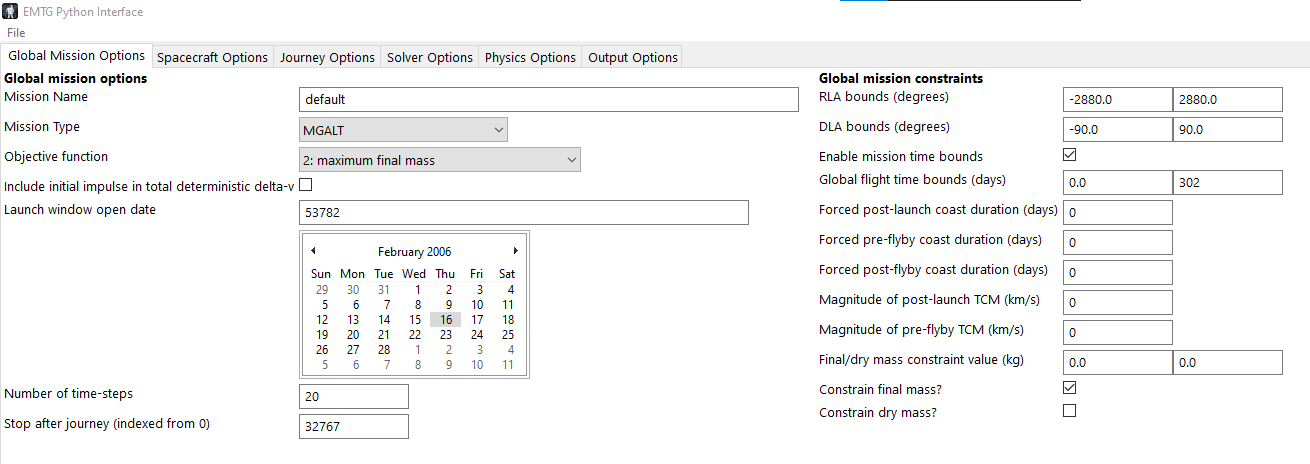
\includegraphics[width=1.0\textwidth]{../../shared_latex_inputs/images/pyemtg_global_options_tab.png}
    \caption{EMTG Global Options tab}
\end{figure}

\subsection{Global Mission Options}

\begin{enumerate}

    \item \textbf{Mission Name:} The mission name is used to distinguish \ac{EMTG} missions and will prefix the output directories and files \ac{EMTG} produces when a mission is run.

        \begin{table}[H]
            \hspace{2cm}
            \begin{tabular}{ll}
            Data Type & \verb|string| \\
            Default Value & ``default'' \\
            \end{tabular}
        \end{table}

    \item \textbf{Mission Type:} \ac{EMTG} provides several different Mission Types which control how an \ac{EMTG} mission is modeled. Mission Types come in various levels of fidelity and may be selected for the entire mission or on a per-Journey basis. Mission Types are covered in more detail in Chapter~\ref{chap:mission_types}.
        \begin{table}[H]
            \hspace{2cm}
            \begin{tabular}{lp{3cm}}
            Data Type & \verb|PhaseType| \\
            Allowed Values & \verb|MGALT, FBLT, PSBI, PSFB, MGAnDSMs, CoastPhase,| \newline
                             \verb|SundmanCoastPhase, Variable phase type,| \newline
                             \verb|ProbeEntryPhase, ControlLawThrustPhase| \\
            Default Value & \verb|MGALT| \\
            \end{tabular}
        \end{table}

    \item \textbf{Objective Function:} This option specifies the mission parameter to be maximized or minimized such as maximizing final mass or minimizing delta-v.
    
        \begin{table}[H]
            \hspace{2cm}
            \begin{tabular}{lp{5cm}}
            Data Type & \verb|PhaseType| \\
            Allowed Values & \verb|0: minimum deterministic deltaV,| \newline
                             \verb|1: minimum time,| \newline
                             \verb|2: maximum final mass,| \newline
                             \verb|3: maximize initial mass,| \newline
                             \verb|4: depart as late as possible,| \newline
                             \verb|5: depart as early as possible,| \newline
                             \verb|6: maximize orbit energy,| \newline
                             \verb|7: minimize launch mass,| \newline
                             \verb|8: arrive as early as possible,| \newline
                             \verb|9: arrive as late as possible,| \newline
                             \verb|10: minimum propellant,| \newline
                             \verb|11: maximum dry/wet ratio,| \newline
                             \verb|12: maximum arrival kinetic energy,| \newline
                             \verb|13: minimum BOL power,| \newline
                             \verb|14: maximize log\_10(final mass),| \newline
                             \verb|15: maximize log\_e(final mass),| \newline
                             \verb|16: maximum dry mass margin,| \newline
                             \verb|17: maximum dry mass,| \newline
                             \verb|18: maximum log\_10(dry mass),| \newline
                             \verb|19: maximum log\_e(dry mass),| \newline
                             \verb|20: minimize chemical fuel,| \newline
                             \verb|21: minimize chemical oxidizer,| \newline
                             \verb|22: minimize electric propellant,| \newline
                             \verb|23: minimize total propellant,| \newline
                             \verb|24: minimize waypoint tracking error,| \newline
                             \verb|25: minimize initial impulse magnitude,| \newline
                             \verb|26: maximize distance from central body| \\
            Default Value & \verb|2: maximum final mass| \\
            \end{tabular}
        \end{table}

    \item \textbf{Include initial impulse in total deterministic delta-v:} This options controls whether or not the delta-v provided by the launch vehicle is included in the objective function, ``0: minimum deterministic deltaV.''
        
        \begin{table}[H]
            \hspace{2cm}
            \begin{tabular}{ll}
            Data Type & \verb|bool| \\
            Allowed Values & true, false \\
            Default Value & false \\
            Units & NA
            \end{tabular}
        \end{table}

    \item \textbf{Launch window open date:} The earliest possible launch date expressed as an MJD2000 value. This value can be set using the text box or the calendar tool below.
    
        \begin{table}[H]
            \hspace{2cm}
            \begin{tabular}{ll}
            Data Type & \verb|double| \\
            Allowed Values & 0 $<$ Real $<$ $\infty$ \\
            Default Value & 0.0 \\
            Units & days since MJD2000 epoch
            \end{tabular}
        \end{table}
    
    \item \textbf{Number of time-steps:} Number of time-steps per journey/phase. This controls how many segments define each Journey. A higher value increases the mission fidelity at the cost of run time. This option can be overridden on a per-Journey basis in the Journey Options tab.
    
        \begin{table}[H]
            \hspace{2cm}
            \begin{tabular}{ll}
            Data Type & \verb|int| \\
            Allowed Values & 0 $<$ Integer $<$ $\infty$ \\
            Default Value & 20 \\
            Units & NA
            \end{tabular}
        \end{table}
        
    \item \textbf{Stop after journey (indexed from 0):} This will cause \ac{EMTG} to only optimize up to and including the integer Journey number set in the text box. For example, if the \ac{EMTG} Options file has 3 Journeys (Journey 0 to Journey 2) and this text box is set to 1, \ac{EMTG} will not solve Journey 2.

        \begin{table}[H]
            \hspace{2cm}
            \begin{tabular}{ll}
            Data Type & \verb|int| \\
            Allowed Values & 0 $<$ Integer $<$ (Number of Journeys - 1) \\
            Default Value & 32767 \\
            Units & NA
            \end{tabular}
        \end{table}
    

\end{enumerate}
    
\subsection{Global Mission Constraints}

\begin{enumerate}
    \item \textbf{RLA bounds (degrees):} Bound the right ascension of the launch asymptote (equatorial east longitude from the vernal equinox).

        \begin{table}[H]
            \hspace{2cm}
            \begin{tabular}{ll}
            Data Type & \verb|std::vector<double, 2>| \\
            Allowed Values & -$\infty$ $<$ Real $<$ $\infty$ \\
            Default Value & [-2880.0, 2880.0] \\
            Units & degrees
            \end{tabular}
        \end{table}

    \item \textbf{\acs{DLA} bounds (degrees):} Bound the declination (latitude) of the launch asymptote. 
    
        \begin{table}[H]
            \hspace{2cm}
            \begin{tabular}{ll}
            Data Type & \verb|std::vector<double, 2>| \\
            Allowed Values & -90 $<$ Real $<$ 90 \\
            Default Value & [-90.0, 90.0] \\
            Units & degrees
            \end{tabular}
        \end{table}

    \item \textbf{Enable mission time bounds:} Selecting this box will reveal the Global flight time upper and lower bounds boxes to constrain the mission length.
    
        \begin{table}[H]
            \hspace{2cm}
            \begin{tabular}{ll}
            Data Type & \verb|bool| \\
            Allowed Values & true, false \\
            Default Value & true \\
            Units & NA
            \end{tabular}
        \end{table}

    \item \textbf{Global flight time bounds (days):} Used to set boundaries on mission length in days where 0.0 is the launch epoch. Revealed and active only if "Enable mission time bounds" is checked.
    
        \begin{table}[H]
            \hspace{2cm}
            \begin{tabular}{ll}
            Data Type & \verb|std::vector<double, 2>| \\
            Allowed Values & 0 $<$ Real $<$ $\infty$ \\
            Default Value & [0, 302] \\
            Units & days
            \end{tabular}
        \end{table}

    \item \textbf{Forced post-launch coast duration (days):} Restrict \ac{EMTG} from placing any maneuvers between launch and this option's value in days. This can be used to ensure adequate time for spacecraft checkout after launch.
    
        \begin{table}[H]
            \hspace{2cm}
            \begin{tabular}{ll}
            Data Type & \verb|double| \\
            Allowed Values & 0 $<$ Real $<$ $\infty$ \\
            Default Value & 0.0 \\
            Units & days
            \end{tabular}
        \end{table}

    \item \textbf{Forced pre-flyby coast duration (days):} Restrict \ac{EMTG} from placing any maneuvers this many days prior to a planetary flyby. This can be used to ensure adequate time for trajectory error cleanup prior to the flyby.
    
        \begin{table}[H]
            \hspace{2cm}
            \begin{tabular}{ll}
            Data Type & \verb|double| \\
            Allowed Values & 0 $<$ Real $<$ $\infty$ \\
            Default Value & 0.0 \\
            Units & days
            \end{tabular}
        \end{table}

    \item \textbf{Forced post-flyby coast duration (days):} Restrict \ac{EMTG} from placing any maneuvers this many days after a planetary flyby.
    
        \begin{table}[H]
            \hspace{2cm}
            \begin{tabular}{ll}
            Data Type & \verb|double| \\
            Allowed Values & 0 $<$ Real $<$ $\infty$ \\
            Default Value & 0.0 \\
            Units & days
            \end{tabular}
        \end{table}

    \item \textbf{Magnitude of post-launch TCM (km/s):} Sets the upper bound on a post-launch TCM. \ac{EMTG} sets the lower bound to 0 km/s internally. The post-launch TCM is assumed to be performed by the monopropellant propulsion system and is used to compute the mass loss due to the TCM on the left boundary of a phase.
    
        \begin{table}[H]
            \hspace{2cm}
            \begin{tabular}{ll}
            Data Type & \verb|double| \\
            Allowed Values & 0 $<$ Real $<$ $\infty$ \\
            Default Value & 0.0 \\
            Units & km/s
            \end{tabular}
        \end{table}

    \item \textbf{Magnitude of pre-flyby TCM (km/s):} Sets the upper bound on a pre-flyby TCM. \ac{EMTG} sets the lower bound to 0 km/s internally. The pre-flyby TCM is assumed to be performed by the monopropellant propulson system and is used to compute the mass loss due to TCM immediately before a flyby.

        \begin{table}[H]
            \hspace{2cm}
            \begin{tabular}{ll}
            Data Type & \verb|double| \\
            Allowed Values & 0 $<$ Real $<$ $\infty$ \\
            Default Value & 0.0 \\
            Units & km/s
            \end{tabular}
        \end{table}

    \item \textbf{Constrain final/dry mass?:} Checking either of these options reveals a set of text boxes to bound either the final mass or the dry mass of the spacecraft at the end of the mission. Final mass is also known as final wet (including propellant) mass. These options are applied separately, allowing users to constrain both the vehicle dry mass and the final mission mass at the same time. 

        \begin{table}[H]
            \hspace{2cm}
            \begin{tabular}{ll}
            Data Type & bool \\
            Allowed Values & true, false \\
            Default Value & false \\
            Units & NA
            \end{tabular}
        \end{table}

    \item \textbf{Final/dry mass constraint value (kg):} Mass values for the final/dry mass constraint. Revealed and active only if either the constrain final or dry mass is active.
    
        \begin{table}[H]
            \hspace{2cm}
            \begin{tabular}{ll}
            Data Type & \verb|std::vector<double, 2>| \\
            Allowed Values & 0 $<$ Real $<$ $\infty$ \\
            Default Value & [0.0, 0.0] \\
            Units & kg
            \end{tabular}
        \end{table}

\end{enumerate}